\documentclass[main.tex]{subfiles}

\begin{document}

\section{Landmarks}

Before implementing that uses Landmarks, the options first have to be analysed as to whether they can provide the benefits in our specific environment. The main options that were explored were:

\begin{itemize}
	\item Stairs
	\item Elevator
	\item Areas of unique magnetic readings
	\item Wi-fi Routers
\end{itemize}

The first 2 options are present in the department building, so there are available for use. However they are limited in how they can help with resetting the error in the system, this is because these are only used when a user will move from floor to floor. Meaning navigation on a single floor will not be helped with resetting error but over multiple they can be used to that effect. 

For detecting these there are unique patterns from the accelerometer readings and in conjunction with the potential for the barometer to verify the movement between floors they can be used as Landmarks. However a detection algorithm did not get implement for these, and to help with the issue of error building up the user simply alerts the application that they have transitioned up or down a floor on their route.

The third option is more problematic in our environment as the entire building has lots of electronic equipment, such as computers, servers, etc.... This means that there is lots of magnetic inteference throughout the department, so there is not really any area that has a unique reading that can be used as a Landmark.

This leaves the final option as the only method of removing error when navigating within a floor, to do this all the routers on a floor need to be identified.

\begin{center}
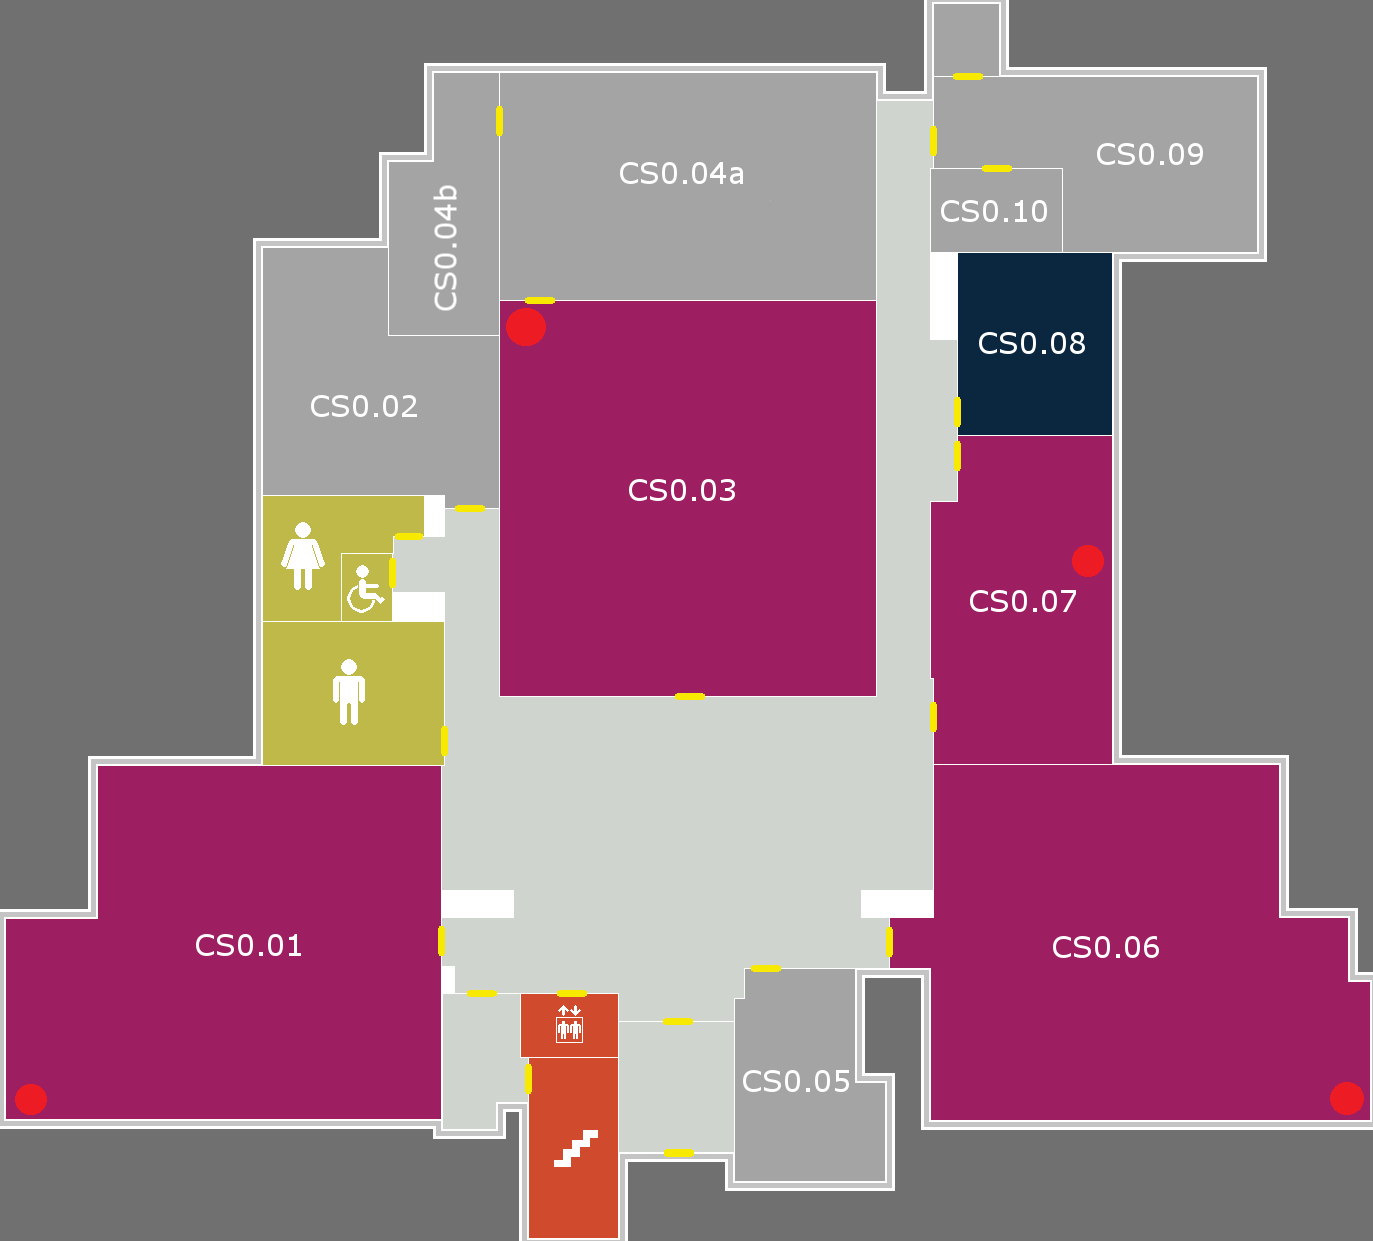
\includegraphics[scale=0.3]{images-implementation/wifiLocation.png}
\captionof{figure}{The location of Wifi routers on the ground floor of DCS, marked as red dots}
\label{fig:wifiLoc}
\end{center}

The locations of these routers unfortunately mean that the usage of them will provide no benefit, shown in Figure~\ref{fig:wifiLoc}. They reside with in the corners of the rooms, and for a landmark to be useful the user must path close enough to it for it to be a viable choice for resetting error. With their locations it is impossible for an effecient routing algorithm to return a path in which the routers are not either at the start or the end of the route. Hence making them effectively useless for this purpose.

We also found that we often picked up routers from different floors in certian areas, which could easily be misinterpreted as the user being someone they are not. As well as this devices would connect to a room's router outside of them, meaning that connecting to a router that is specific to a large room it is an unreliable to assume the user is within it.

Whilst routers are not viable for landmarks on the ground floor for the reasons stated above, it doesn't mean they will not be viable for the upper floors. This was tested the same as before by identifying router locations, but it became quickly evident that from placement again they would not be of use. In conjunction with the large number of small rooms/offices on the upper floors it becomes hard to snap a user to these routers.

Another thing to note about using routers is that there are two main bands that are used for communication, 2Ghz and 5Ghz, so dependent on the routers and smartphones they may not be usable. In this case the router is dualband meaning both are available, it does however mean that 2 MAC addresses are needed to be stored per router for unique identification.

Overall having looked at these landmarks it is clear that at least three of these options could be viable, however in our environment they can't provide their fully inteded benefit.

\section{Barometer}

For the barometer, both Andriod and iOS have native ways to get both the current air pressure and the height above sea level the device is at based off the air pressure. From research and small amounts of testing it was evident that using the absolute height would not provide any useful way of detecting floor change with the fluctuations that occur with time, weather and location. To counter this the difference between heights can be used to detect if a user has gone up or down a floor. 

However despite there being a clear correlation between moving between floors and the change in height, the values from recieved from these native functions would range between 3-5 values over a small period of time. This means that it is very difficult to be certain if the user has changed floors or it is simply an outlier from the functions. 

To help combat this the average was taken over a large number of reading across a period of time, however whilst this solved the rapidly changing value, it meant that if a user took to long transistioning between floors the average would slowly slide in their direction fo movement. When this occurs nothing will be flagged as a large enough distance to be moving from floor A to B and the system recognise the movement. 

Given more time this issues could be solved, and from research and the testing done it can be seen that the barometer will be a useful sensor for inddor localisation.

\end{document}